\documentclass{article}
\usepackage{tikz}
\usepackage[margin=0.5in]{geometry}
\begin{document}
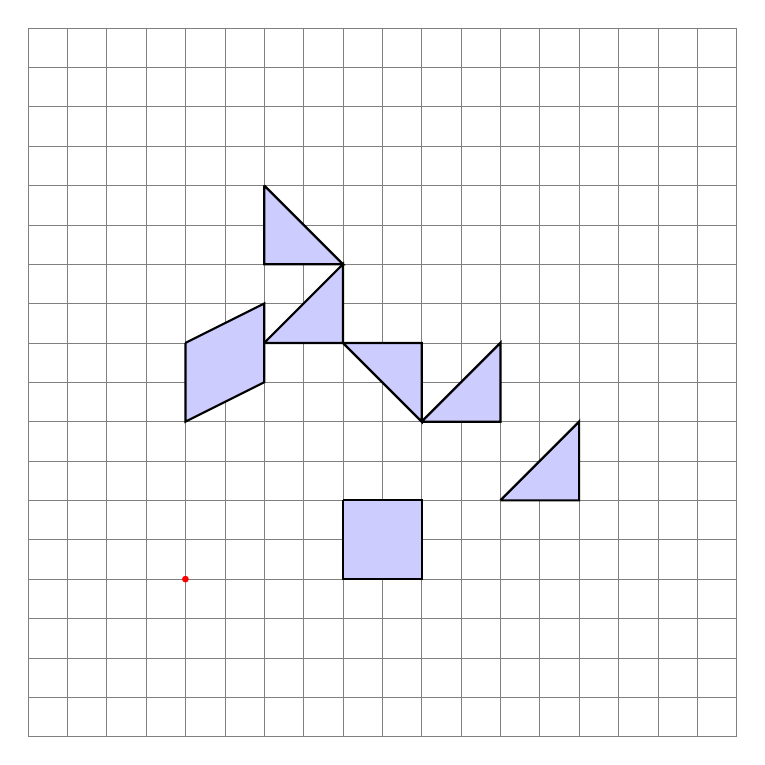
\begin{tikzpicture}[scale=1]
  \draw[step=5mm,gray,very thin] (-2.0,-2.0) grid (7.0,7.0);
  \filldraw[red] (0,0) circle (1pt);
  \draw[thick, fill=blue!20] (1.0,3.0) -- (2.0,3.0) -- (2.0,4.0) -- (1.0,3.0);
  \draw[thick, fill=blue!20] (4.0,1.0) -- (5.0,2.0) -- (5.0,1.0) -- (4.0,1.0);
  \draw[thick, fill=blue!20] (3.0,2.0) -- (4.0,3.0) -- (4.0,2.0) -- (3.0,2.0);
  \draw[thick, fill=blue!20] (1.0,5.0) -- (1.0,4.0) -- (2.0,4.0) -- (1.0,5.0);
  \draw[thick, fill=blue!20] (2.0,3.0) -- (3.0,2.0) -- (3.0,3.0) -- (2.0,3.0);
  \draw[thick, fill=blue!20] (2.0,1.0) -- (2.0,0.0) -- (3.0,0.0) -- (3.0,1.0) -- (2.0,1.0);
  \draw[thick, fill=blue!20] (0.0,3.0) -- (1.0,3.5) -- (1.0,2.5) -- (0.0,2.0) -- (0.0,3.0);
\end{tikzpicture}
\end{document}
